% A LaTeX (non-official) template for ISAE projects reports
% Copyright (C) 2014 Damien Roque
% Version: 0.2
% Author: Damien Roque <damien.roque_AT_isae.fr>

\documentclass[a4paper,12pt]{article}
\usepackage[utf8]{inputenc}
\usepackage[T1]{fontenc}
\usepackage[frenchb]{babel} % If you write in French
\usepackage{graphicx}
\usepackage{subfig}
\usepackage{tikz}
\usetikzlibrary{shapes,arrows}
\usepackage{pgfplots}
\pgfplotsset{compat=newest}
\pgfplotsset{plot coordinates/math parser=false}
\newlength\figureheight
\newlength\figurewidth
\pgfkeys{/pgf/number format/.cd,
set decimal separator={,\!},
1000 sep={\,},
}
\usepackage{ifthen}
\usepackage{ifpdf}
\ifpdf
\usepackage[pdftex]{hyperref}
\else
\usepackage{hyperref}
\fi
\usepackage{color}
\hypersetup{%
colorlinks=true,
linkcolor=black,
citecolor=black,
urlcolor=black}

\renewcommand{\baselinestretch}{1.05}
\usepackage{fancyhdr}
\pagestyle{fancy}
\fancyfoot{}
\fancyhead[LE,RO]{\bfseries\thepage}
\fancyhead[RE]{\bfseries\nouppercase{\leftmark}}
\fancyhead[LO]{\bfseries\nouppercase{\rightmark}}
\setlength{\headheight}{15pt}

\let\headruleORIG\headrule
\renewcommand{\headrule}{\color{black} \headruleORIG}
\renewcommand{\headrulewidth}{1.0pt}
\usepackage{colortbl}
\arrayrulecolor{black}

\fancypagestyle{plain}{
  \fancyhead{}
  \fancyfoot[C]{\thepage}
  \renewcommand{\headrulewidth}{0pt}
}

\makeatletter
\def\@textbottom{\vskip \z@ \@plus 1pt}
\let\@texttop\relax
\makeatother

\makeatletter
\def\cleardoublepage{\clearpage}
\makeatother

\usepackage{amsthm}
\usepackage{amssymb,amsmath,bbm}
\usepackage{array}
\usepackage{bm}
\usepackage{multirow}
\usepackage[footnote]{acronym}

\newcommand*{\SET}[1]  {\ensuremath{\mathbf{#1}}}
\newcommand*{\VEC}[1]  {\ensuremath{\boldsymbol{#1}}}
\newcommand*{\FAM}[1]  {\ensuremath{\boldsymbol{#1}}}
\newcommand*{\MAT}[1]  {\ensuremath{\boldsymbol{#1}}}
\newcommand*{\OP}[1]  {\ensuremath{\mathrm{#1}}}
\newcommand*{\NORM}[1]  {\ensuremath{\left\|#1\right\|}}
\newcommand*{\DPR}[2]  {\ensuremath{\left \langle #1,#2 \right \rangle}}
\newcommand*{\calbf}[1]  {\ensuremath{\boldsymbol{\mathcal{#1}}}}
\newcommand*{\shift}[1]  {\ensuremath{\boldsymbol{#1}}}

\newcommand{\eqdef}{\stackrel{\mathrm{def}}{=}}
\newcommand{\argmax}{\operatornamewithlimits{argmax}}
\newcommand{\argmin}{\operatornamewithlimits{argmin}}
\newcommand{\ud}{\, \mathrm{d}}
\newcommand{\vect}{\text{Vect}}
\newcommand{\sinc}{\ensuremath{\mathrm{sinc}}}
\newcommand{\esp}{\ensuremath{\mathbb{E}}}
\newcommand{\hilbert}{\ensuremath{\mathcal{H}}}
\newcommand{\fourier}{\ensuremath{\mathcal{F}}}
\newcommand{\sgn}{\text{sgn}}
\newcommand{\intTT}{\int_{-T}^{T}}
\newcommand{\intT}{\int_{-\frac{T}{2}}^{\frac{T}{2}}}
\newcommand{\intinf}{\int_{-\infty}^{+\infty}}
\newcommand{\Sh}{\ensuremath{\boldsymbol{S}}}
\newcommand{\C}{\SET{C}}
\newcommand{\R}{\SET{R}}
\newcommand{\Z}{\SET{Z}}
\newcommand{\N}{\SET{N}}
\newcommand{\K}{\SET{K}}
\newcommand{\reel}{\mathcal{R}}
\newcommand{\imag}{\mathcal{I}}
\newcommand{\cmnr}{c_{m,n}^\reel}
\newcommand{\cmni}{c_{m,n}^\imag}
\newcommand{\cnr}{c_{n}^\reel}
\newcommand{\cni}{c_{n}^\imag}
\newcommand{\tproto}{g}
\newcommand{\rproto}{\check{g}}
\newcommand{\LR}{\mathcal{L}_2(\SET{R})}
\newcommand{\LZ}{\ell_2(\SET{Z})}
\newcommand{\LZI}[1]{\ell_2(\SET{#1})}
\newcommand{\LZZ}{\ell_2(\SET{Z}^2)}
\newcommand{\diag}{\operatorname{diag}}
\newcommand{\noise}{z}
\newcommand{\Noise}{Z}
\newcommand{\filtnoise}{\zeta}
\newcommand{\tp}{g}
\newcommand{\rp}{\check{g}}
\newcommand{\TP}{G}
\newcommand{\RP}{\check{G}}
\newcommand{\dmin}{d_{\mathrm{min}}}
\newcommand{\Dmin}{D_{\mathrm{min}}}
\newcommand{\Image}{\ensuremath{\text{Im}}}
\newcommand{\Span}{\ensuremath{\text{Span}}}

\newtheoremstyle{break}
  {11pt}{11pt}%
  {\itshape}{}%
  {\bfseries}{}%
  {\newline}{}%
\theoremstyle{break}

\usetikzlibrary{arrows,shapes,snakes,automata,backgrounds,petri}
\newcommand{\hsp}{\hspace{20pt}}
\newcommand{\HRule}{\rule{\linewidth}{0.5mm}}



\title{ON : Rapport Projet}
\author{XAMBILI Robin}

\date{}


%Debut de ton document
\begin{document}
\makeatletter
  \begin{titlepage}
  \centering
      {\large \textsc{École Nationale Supérieure \\ d'Électrotechnique, d'Électronique, d'Informatique, \\ d'Hydraulique et des Télécommunications}}\\ \vspace{0.50cm}
      \textsc{Institut National Polytechnique}\\
    \vspace{1cm}
      
\includegraphics[width=0.7\textwidth]{img/n7.jpg}
  
    \vspace{3.5cm}
   % Title
    \HRule \\[0.3cm]
    { \huge \bfseries Optimisation Numérique : \\ \vspace{3mm} Rapport Projet \\ 
    }
    \HRule \\[2cm]
    \vfill
    % Author
    \vspace{2em}
             
    \large XAMBILI Robin
    \vfill
	% Bas de page
	%\textsc{6 Novembre 2017}
    \newpage
    \renewcommand{\contentsname}{SOMMAIRE}
    \tableofcontents
  \end{titlepage}

%%%%%%%%%%%%%%%%%%%%%%%%%%%%%%%%%%%%%%%%%%%%
%%% Content of the report and references %%%
%%%%%%%%%%%%%%%%%%%%%%%%%%%%%%%%%%%%%%%%%%%%

\section{Introduction}

La première partie de ce TP-projet concerne les problèmes d'optimisation sans contraintes. On étudie la méthode de Newton et sa globalisation par l'algorithme des régions de confiance. La résolution du sous-problème des régions de confiance sera réalisée de deux façons, soit à l'aide du point de Cauchy, soit par l'algorithme de Moré-Sorensen.
La seconde partie du projet exploite la partie précédente pour résoudre des problèmes d'optimisation avec contraintes par l'algorithme du Lagrangien augmenté.
\newpage
\section{Algorithme de Newton Local}
\subsection{Présentation}

La fonction f étant $C^2$, on peut remplacer f au voisinage de l’iteré courant $x_k$ par son
développement de Taylor au second ordre, soit :\\
$q(y) = f(x_k) + \nabla f(x_k)^T (y-x_k) + 1/2 (y-x_k)^T \nabla^2 f(x_k) (y-x_k)$.

Lorsque la matrice hessienne de la fonction est définie positive en $x_k$, une itération de la méthode de Newton locale revient à minimiser le modèle quadratique de la fonction en $x_k$.

Cela revient donc à trouver x qui vérifie : $\nabla q(x) = 0$ , soit :\\
$x_{k+1} = x_k + d_k$\\
avec $d_k$ unique solution de : \\
$\nabla^2 f(x_k)d_k = - \nabla f(x_k)$


\subsection{Algorithme}

L'algorithme prend en entrée $f, \nabla f, \nabla^2 f, x_0$, tol1 (tolérance de convergence sur le gradient), tol2 (tolérance de stagnation) et itermax et renvoie le minimum x.\\

\textbf{Critère d'arrêt : }
\begin{itemize}
\item convergence du gradient : $||\nabla f(x_k)|| \leq tol1 \times ||\nabla f(x_0)||$,
\item stagnation : $||x_(k+1) - x_k||  \leq tol2$,
\item nombre d'itération : $iter \geq itermax$\\
\end{itemize}

L'algorithme se déroule comme suit :\\
\textbf{Tant que test de convergence non satisfait :}
\begin{enumerate}
	\item calculer $d_k$
	\item mettre à jour $x_k$ et $k$
	\item mettre à jour le test de convergence
\end{enumerate}

\subsection{Tests de l'algorithme}
Les test sont réalisés sur les fonctions $f_1$ et $f_2$ données en annexes (9.1) :
\begin{figure}[htbp]
	\centering
		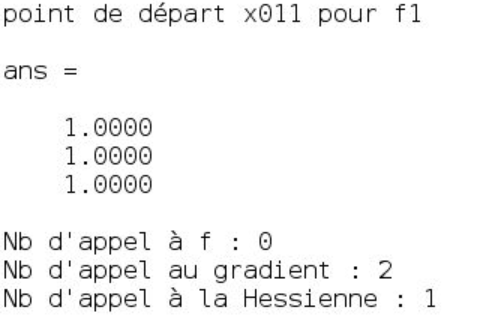
\includegraphics{img/test1_newton.PNG}
\end{figure}
\begin{figure}[htbp]
	\centering
		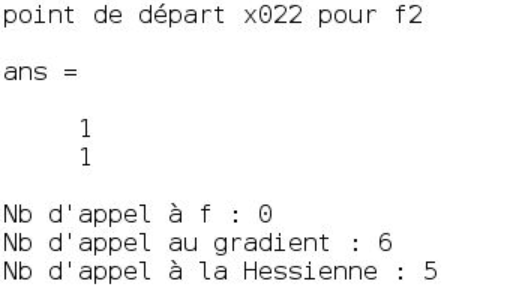
\includegraphics{img/test2_newton.PNG}
\end{figure}
\begin{figure}[htbp]
	\centering
		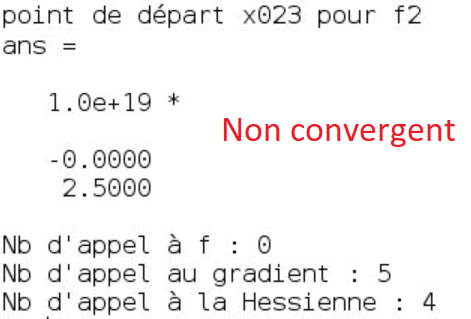
\includegraphics{img/test3_newton.PNG}
\end{figure}


\subsection{Interprétations}
\begin{itemize}
\item[•] $f_1$ converge en une seule itération car c'est une fonction quadratique;
\item[•] $f_2$ converge avec $x_022$ pour point initial cependant elle ne converge pas avec $x_023$ comme point initial;
\item[•] divergence possible si le point de départ est trop éloigné de la solution;
\item[•] vitesse de convergence quadratique dans des conditions favorables.
\end{itemize}

En bref, cette méthode converge rapidement mais la convergence n'est pas garantie et dépend du point de départ choisi .

\newpage

\section{Algorithme des Région de Confiance}
\subsection{Présentation}

L'introduction d'une région de confiance dans la méthode de Newton permet de garantir
la convergence globale de celle-ci, i.e. la convergence vers un optimum local quel que soit
le point de départ. Cela suppose certaines conditions sur la résolution locale des sous-problèmes issus de la méthode, qui sont aisément imposables.

On veut approcher notre fonction $f$ à minimiser par une fonction $m_k$ dans l'espace $R_k = {x_k+s; ||s||<\Delta_k}$ pour un $\Delta_k$ fixé, cette région doit être petite pour que l'approximation $m_k(x_k+s)~f(x_k+s)$ soit vraie.

Un exemple de modèle que l'on peut considérer est l'approximation de Taylor à l'ordre 2 (modèle quadratique) : \\
$m_k(x_k+s) = q_k(s) = f(x_k) + g_k^Ts + \frac{1}{2} s^TH_ks$\\
avec $g_k = \nabla f(x_k)$ et $H_k = \nabla^2 f(x_k)$.

L'astuce est de trouver un point $s_k (<=\Delta_k)$ qui minimise $m_k(x_k+s)$ puis de mettre à jour $x_k$ et $\Delta_k$.

\subsection{Algorithme}

L'algorithme prend en entrée $f, \nabla f, \nabla^2 f, x_0,\Delta_{Max}, \Delta_0, \gamma_1, \gamma_2, \eta_1, \eta_2$, tol1 (tolérance de convergence sur le gradient), tol2 (tolérance de stagnation) et itermax et renvoie le minimum x.\\

\textbf{Critère d'arrêt : }
\begin{itemize}
\item convergence du gradient : $||\nabla f(x_k)|| \leq tol1 \times ||\nabla f(x_0)||$,
\item stagnation : $||x_(k+1) - x_k||  \leq tol2$,
\item nombre d'itération : $iter \geq itermax$\\
\end{itemize}

L'algorithme se déroule comme suit :\\
\textbf{Tant que test de convergence non satisfait :}
\begin{enumerate}
	\item calculer le point $s_k$ soit par la méthode de Cauchy soit par Moré-Sorensen.
	\item calculer $\rho_k = \frac{f(x_k) - f(x_k+s_k)}{m_k(x_k)-m_k(x_k+s_k)}$
	\item mettre à jour $x_{k+1} = \begin{cases}
x_k+s_k &\text{ si }\rho_k\geq\eta_1 \\
x_k &\text{ sinon }
\end{cases}$
	\item Mettre à jour la région de confiance : 
		$\Delta_{k+1} = \begin{cases}
			\min{\gamma_2\Delta_k, \Delta_{max}} &\text{ si }\rho_k\geq\eta_2 \\
			\Delta_k &\text{ si }\rho_k\in[\eta_1,\eta_2)\\
			\gamma_1\Delta_k &\text{ sinon }
		\end{cases}$
	\item on retourne $x_k$
\end{enumerate}

\subsection{Tests de l'algorithme}
Les test sont réalisés sur les fonctions $f_1$ et $f_2$ données en annexes (9.1) avec la méthode du pas de Cauchy:
\begin{figure}[htbp]
	\centering
		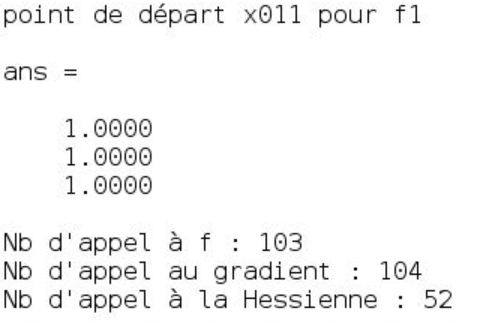
\includegraphics{img/test1_region.PNG}
\end{figure}

\subsection{Interprétations}

On remarque que les appels à $f$, $\nabla f$ et $\nabla^2 f$ sont plus nombreux pour l'algorithme des régions de confiance avec la méthode du pas de Cauchy qu'avec l'algorithme de Newton local. Donc, cette méthode est moins efficace que celle de Newton.

\newpage

\section{Algorithme du Pas de Cauchy}
\subsection{Présentation}

On considère ici le modèle quadratique $q_k(s)$. Le sous-problème de régions de confiance
correspondant peut se révéler difficile à résoudre (parfois autant que le problème de départ).
Il est donc intéressant de se restreindre à une résolution approchée de ce problème.
Le pas de Cauchy appartient à la catégorie des solutions approchées. Il s'agit de se
restreindre au sous-espace engendré par le vecteur $g_k$ ; le sous-problème s'écrit alors :\\
$\begin{cases}
			\min q_k(s) \\
			s = -t*g_k\\
			t > 0 \\
			||s||< \Delta_k
		\end{cases}$

\subsection{Algorithme}

L'algorithme prend en entrée $\nabla_k f, \nabla^2_k f, \Delta$ et renvoie le minimum $s$ du problème ci-dessus.


\subsection{Tests de l'algorithme}
Les test sont réalisés sur les quadratiques données en annexes (9.2):
\begin{figure}[htbp]
	\centering
		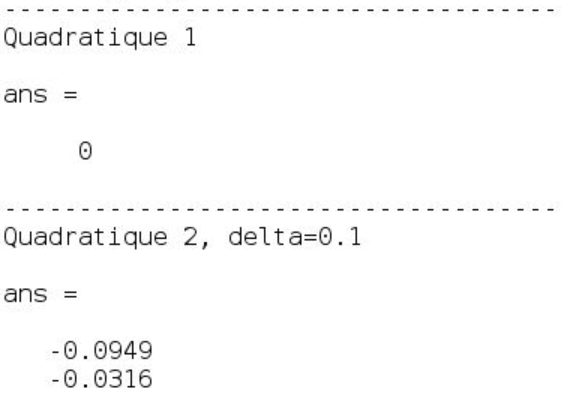
\includegraphics{img/test1_pas_cauchy.PNG}
\end{figure}
\begin{figure}[htbp]
	\centering
		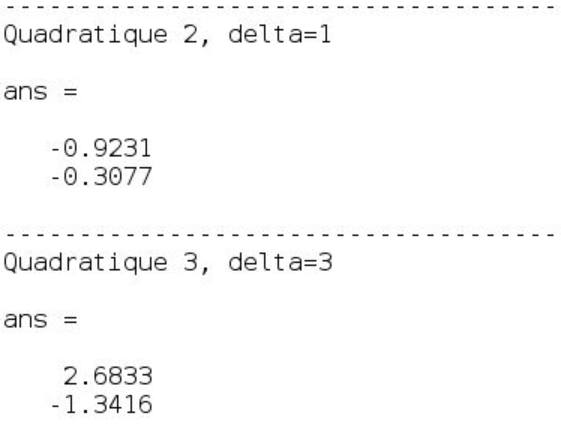
\includegraphics{img/test2_pas_cauchy.PNG}
\end{figure}


\subsection{Interprétations}
Ces tests permettent de valider l'implémentation de l'algorithme du pas de Cauchy.

\newpage

\section{Algorithme de Newton non Linéaire}
\subsection{Présentation}

On voudra par la suite, résoudre des équations de la forme $\phi(\lambda)=0$, où la fonction $\phi$ est une fonction non linéaire de la variable réelle. Cela sera réalisé (de façon approchée) par l'utilisation de la méthode de Newton, combinée avec une technique
de dichotomie pour assurer sa convergence.

\subsection{Algorithme}

L'algorithme prend en entrée $\phi$ (la fonction dont on veut calculer le minimum), $\nabla \phi$ (fonction qui calcule le gradient de la fonction f), $\lambda_{min}$ et $\lambda_{max}$ (valeurs telle que point qui annule $\phi \in [\lambda_{min} ; \lambda_{max}]$), tol (le critère d'arrêt de l'algorithme) et itermax; et renvoie la racine $\lambda$ du problème.\\


\textbf{Critère d'arrêt : }
\begin{itemize}
\item condition d'arrêt : $min(|\phi(\lambda_{min})|, |\phi(\lambda_{max})|) < tol $,
\item nombre d'itération : $iter \geq itermax$\\
\end{itemize}

L'algorithme se déroule comme suit :\\
\begin{enumerate}
	\item Si $min {|\phi(\lambda_min)|, |\phi(\lambda_max)|} < epsilon$, on termine avec la valeur appropriée pour $\lambda^*$; sinon on prend $\lambda = \lambda_max$.
	\item calculer $\lambda^N = \lambda - \frac{\phi(\lambda)}{\phi'(\lambda)}$.
	\item si $\lambda^N \in [\lambda_{min}, \lambda_{max}]$ et $|\phi(\lambda^N)| < \frac{1}{2} |\phi(\lambda)|$, alors $\lambda = \lambda^N$.
	\item sinon calculer $\lambda^D = \frac{\lambda_{min} + \lambda_{max}}{2}$, et on affecte à $\lambda_{min}$ ou $\lambda_{max}$ $\lambda^D$ tel que le produit $\phi(\lambda_{min})*\phi(\lambda_{max}) \leq 0$ reste valide, enfin on affecte $\lambda = \lambda^D$
	\item si le critère d'arrêt est satisfait on sort avec $\lambda^* = \lambda$ sinon on reprend à $\lambda^N$.
\end{enumerate}

\newpage

\subsection{Tests de l'algorithme}
Les test sont réalisés sur les fonctions données en annexes (9.3):
\begin{figure}[htbp]
	\centering
		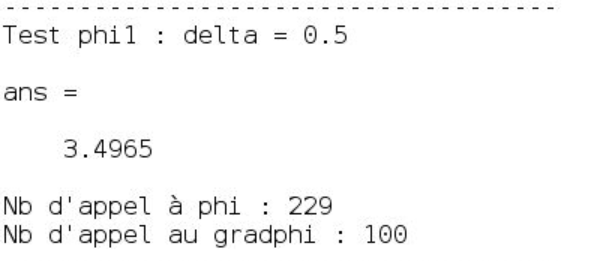
\includegraphics{img/test1_newton_non_lineaire.PNG}
\end{figure}
\begin{figure}[htbp]
	\centering
		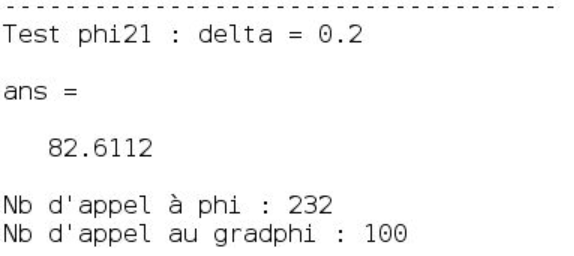
\includegraphics{img/test2_newton_non_lineaire.PNG}
\end{figure}
\begin{figure}[htbp]
	\centering
		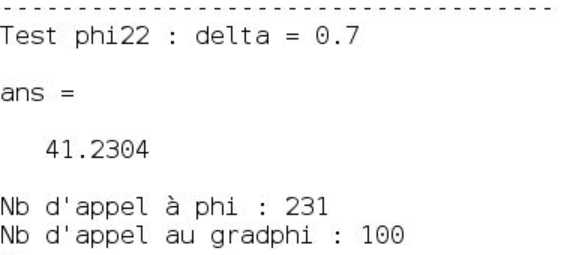
\includegraphics{img/test3_newton_non_lineaire.PNG}
\end{figure}


\subsection{Interprétations}
Si le couple ($\lambda_{min}$, $\lambda_{max}$) fourni par l'utilisateur ne vérifie pas la condition $\phi(\lambda_{min}) \times \phi(\lambda{max}) < 0$ alors il faut envisager un pré-traitement. Ce pré-traitement pourrait consister en incrémentant $\lambda_min$ jusqu'à que la condition soit vérifiée ou $\lambda_min = \lambda_max$, dans ce cas on décrémente $\lambda_min$ jusqu'à que la condition soit vérifiée.

\newpage

\section{Algorithme de Moré-Sorensen}
\subsection{Présentation}

Si s* est solution du problème 
$m_k(x_{k+1}) = \begin{cases}
			\min m_k(x_k+s) \\
			||s||< \Delta_k
		\end{cases}$, avec le modèle quadratique pour approximation de la fonction à minimiser, que l’on représentera de manière générique par $\begin{cases}
			\min g^T s + \frac{1}{2} s^T H s \\
			||s||< \Delta_k
		\end{cases}$, alors il existe $\lambda* \geq 0$ tel que $\begin{cases}
			(H + \lambda*I)s* = -g \\
			\lambda*(||s*|| - \Delta) = 0\\
			H + \lambda*I \succ 0\\
			\lambda* \geq 0\\
			||s*|| \leq \Delta
		\end{cases}$.

La résolution de ce système d’équations passe par la détermination de $\lambda*$.


\newpage

\section{Algorithme du Lagrangien Augmenté}
\subsection{Présentation}

La méthode du lagrangien augmenté appartient à une classe d'algorithmes qui permettent
la résolution des problèmes avec contraintes. Elle s'apparente aux méthodes de
pénalisation, dans lesquelles on résout le problème avec contraintes à travers une suite de
problèmes sans contraintes.

Ici on ne s'intéresse qu'aux problèmes avec contraintes d'égalité c'est à dire : \\ 
$\begin{cases}
			\min f(x) \\
			x \in R^n \\
			c(x)=0,$ où $c: R^n \rightarrow R^m
		\end{cases}$

\subsection{Algorithme}

L'algorithme prend en entrée $f$ (la fonction dont on veut calculer le minimum), $\nabla f$ (fonction qui calcule le gradient de la fonction f), $\nabla^2 f$ (fonction qui calcule la hessienne de la fonction f), $c$ (la fonction qui calcule les contraintes), $J_c$ (la fonction qui calcule la jacobienne des contraintes), $H_c$ (la hessienne de c), $x_0$ (le point de départ de notre algorithme), $\mu_0$ (le paramètre de pénalité), $\tau$ (valeur qui contrôle l'augmentation du paramètre de pénalité), $\lambda_0$ (la valeur initiale du multiplicateur de Lagrange), tol1, tol2, tol3 (les tolérances), itermax et solveur (qui correspond à l'algorithme utilisé pour le sous-problème sans contraintes) et renvoie le minimum $x$ du problème ci-dessus, $\lambda$ le multiplicateur de Lagrange associé aux contraintes d'égalité et $\mu$ le paramètre de pénalité.


\textbf{Critère d'arrêt : }
\begin{itemize}
\item CN1 : $||\nabla La(x_k)|| \leq tol1 \&\& ||c(x_k)|| \leq tol2$,
\item stagnation : $||x_(k+1) - x_k||  \leq tol3 \&\& ||c(x_k)|| \leq tol2$,
\item nombre d'itération : $iter \geq itermax$\\
\end{itemize}

L'algorithme se déroule comme suit :\\
\textbf{Tant que test de convergence non satisfait :}
\begin{enumerate}
	\item on initialise les paramètres initiaux.
	\item on résout avec les algorithmes vus précédemment le problèmes sans contraintes suivant : (avec $x_k$ comme point de départ) \\
	 $ \min L_A(x, \lambda_k, \mu_k) = f(x) + \lambda_k^T c(x) + \frac{\mu_k}{2} ||c(x)||^2$
	\item on met à jour le test de convergence et on s'arrête si il y a convergence
	\item sinon si $||c(x_{k+1})|| \leq \eta_k$ on met à jours les multiplicateurs : \\
	$\begin{cases}
			\lambda_{k+1} = \lambda_k + \mu_k c(x_{k+1})\\
			\mu_{k+1} = \mu_k\\
			\epsilon_{k+1} = \frac{\epsilon_k}{\mu_k}\\
			\eta_{k+1} = \frac{\eta_k}{\mu_k^{\beta}} \\
			k = k+1
		\end{cases}$
	\item sinon on met à jour le paramètre de pénalité : \\
	$\begin{cases}
			\lambda_{k+1} = \lambda_k \\
			\mu_{k+1} = \tau * \mu_k\\
			\epsilon_{k+1} = \frac{\epsilon_0}{\mu_{k+1}}\\
			\eta_{k+1} = \frac{\hat{\eta}_0}{\mu_{k+1}^{\alpha}} \\
			k = k+1
		\end{cases}$
\end{enumerate}

\subsection{Tests de l'algorithme}
Les tests sont réalisés sur les fonctions $f_1$ et $f_2$ données en annexe (9.5) avec l'algorithme de Newton local pour le sous-problème sans contraintes
\begin{figure}[htbp]
	\centering
		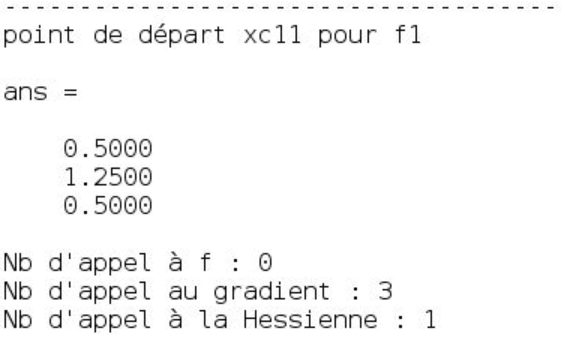
\includegraphics{img/test1_lagrangien_aug.PNG}
\end{figure}
\begin{figure}[htbp]
	\centering
		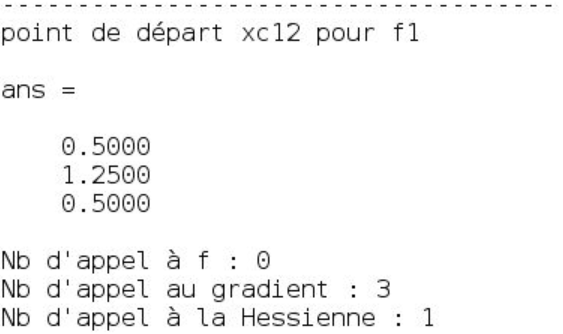
\includegraphics{img/test2_lagrangien_aug.PNG}
\end{figure}

\newpage
\subsection{Interprétations}
On retrouve une convergence en une seule itération puisqu'on utilise Newton local

\newpage

\section{Annexes : Problèmes et cas tests}

\subsection{Problèmes sans contraintes}
\begin{figure}[htbp]
	\centering
		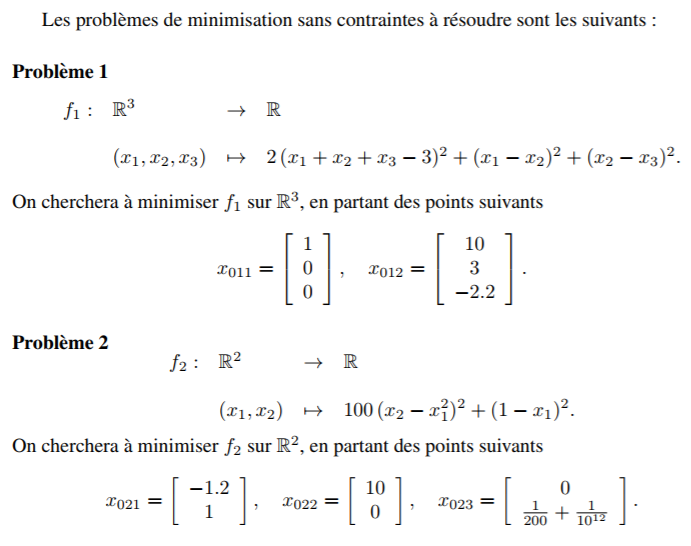
\includegraphics{img/problemes_sans_contraintes.PNG}
\end{figure}

\subsection{Cas tests pour le calcul du pas de Cauchy}
\begin{figure}[htbp]
	\centering
		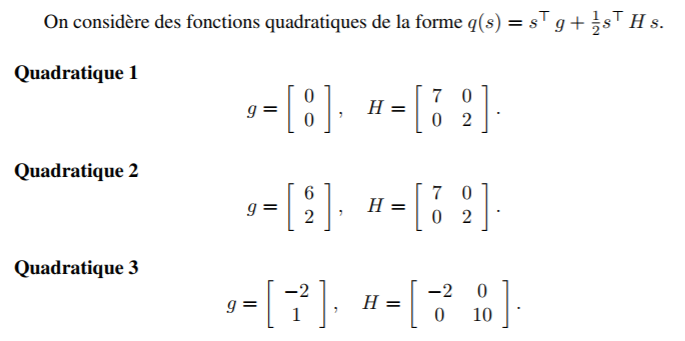
\includegraphics[height=5cm]{img/cas_tests_pas_cauchy.PNG}
\end{figure}

\subsection{Fonctions tests pour l'algorithme de résolution d'équations non linéaires}
\begin{figure}[htbp]
	\centering
		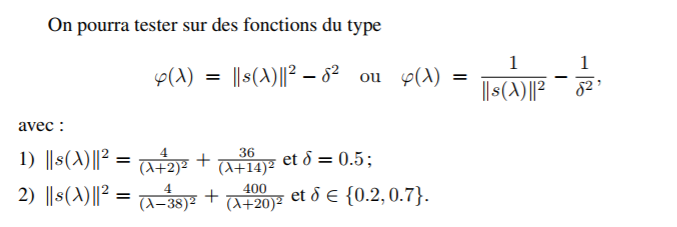
\includegraphics{img/tests_newton_non_lineaire.PNG}
\end{figure}


\subsection{Cas tests pour l'algorithme de Moré-Sorensen}
\begin{figure}[htbp]
	\centering
		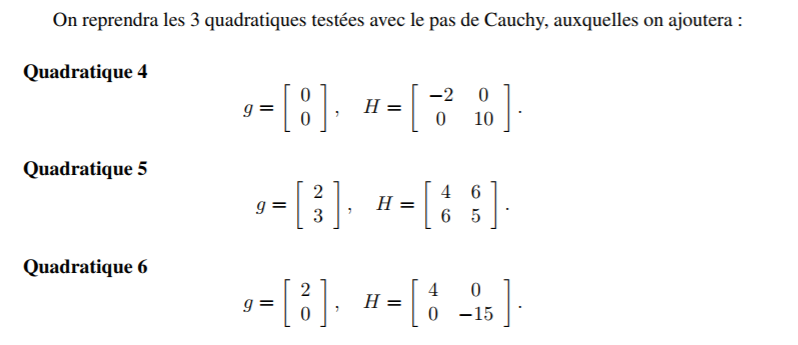
\includegraphics{img/cas_tests_more_sorensen.PNG}
\end{figure}

\newpage

\subsection{Problèmes avec contraintes}
\begin{figure}[htbp]
	\centering
		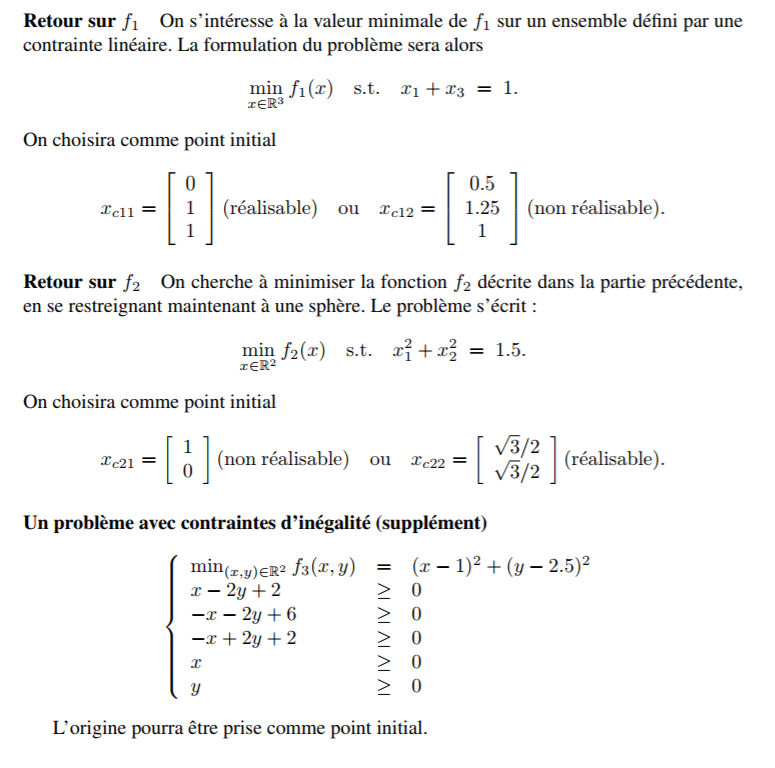
\includegraphics{img/problemes_avec_contraintes.PNG}
\end{figure}

\end{document}